\chapter{Аналитический обзор современного состояния исследований в предметной области}\label{ch:ch1}

\section{Определения рамок обзора}\label{sec:ch1/sec1}

\section{Предпосылки появления модульного оборудования}

\subsection{Многофункциональные универсальные металлорежущие станки}

Многофункциональные универсальные станки появились в начале 20 века и сочетали в себе различные функциональные возможности по обработке металлических заготовок. Все функциональные блоки размещались на одной станине и в зависимости от потребностей производства могли устанавливаться или сниматься, формируя различные конфигурации оборудования. Отличительной особенностью подобных станков была возможность работы на одном станке нескольких рабочих одновременно.

В качестве примеров подобного оборудования можно привести следующие многофункциональные универсальные станки:

\paragraph{Dalton Combinantion Machine}

Dalton Combinantion Machine или <<Комбинированный станок>> Далтона представлял собой большой и тяжелый станок, основанный на стандартной станине и суппорте токарного станка Dalton; эта модель появилась в феврале 1923 года и была защищена многочисленными патентами. Станок первоначально позиционировался как <<представляющий особый интерес для владельцев гаражей и пароходов>> и, как утверждалось, занимал <<пятую часть площади, занимаемой отдельными станками того же типа>>. Несмотря на большое количество обрабатывающих модулей использовать все комбинации сразу на Далтоне было непрактично. Основой конструкции был 13-дюймовый токарно-винторезный станок, на который со стороны передней бабки крепились модули, реализующие функции горизонтально-фрезерного станка с приводным столом размером 24 x 7,5 дюйма, и комбинированного вертикально-фрезерного с пинолью для сверления. 

Самой оригинальной особенностью станка было устройство, с помощью которого мощность подавалась на вертикальные фрезерную и сверлильную головки. В сочетании с коническим шкивом передней бабки, задним редуктором и встроенной коробкой передач, это устройство могло дать фрезерной и сверлильной головке до восемнадцати скоростей. Верхняя часть опоры оправки для горизонтального фрезерного станка была сделана так, чтобы проходить через верхнюю часть передней бабки и, таким образом, в некоторой степени укрепляла конструкцию.

Токарный станок имел межцентровое расстояние равное 37 дюймов в версии со стандартной станиной и 73 дюйма при реализации на длинной станине. Причем последняя поддерживалась третьей опорой, расположенной между двумя внешними. Шпиндель с подшипником из фосфористой бронзы с конусом Морзе имел шесть скоростей, от 20 до 441 об/мин, проходное отверстие диаметром 11/16 дюйма. При этом вся эта <<модульная система>> работала от одного двигателя мощностью 1,5~л.\:с.

\begin{figure}[ht]
	\centerfloat{
		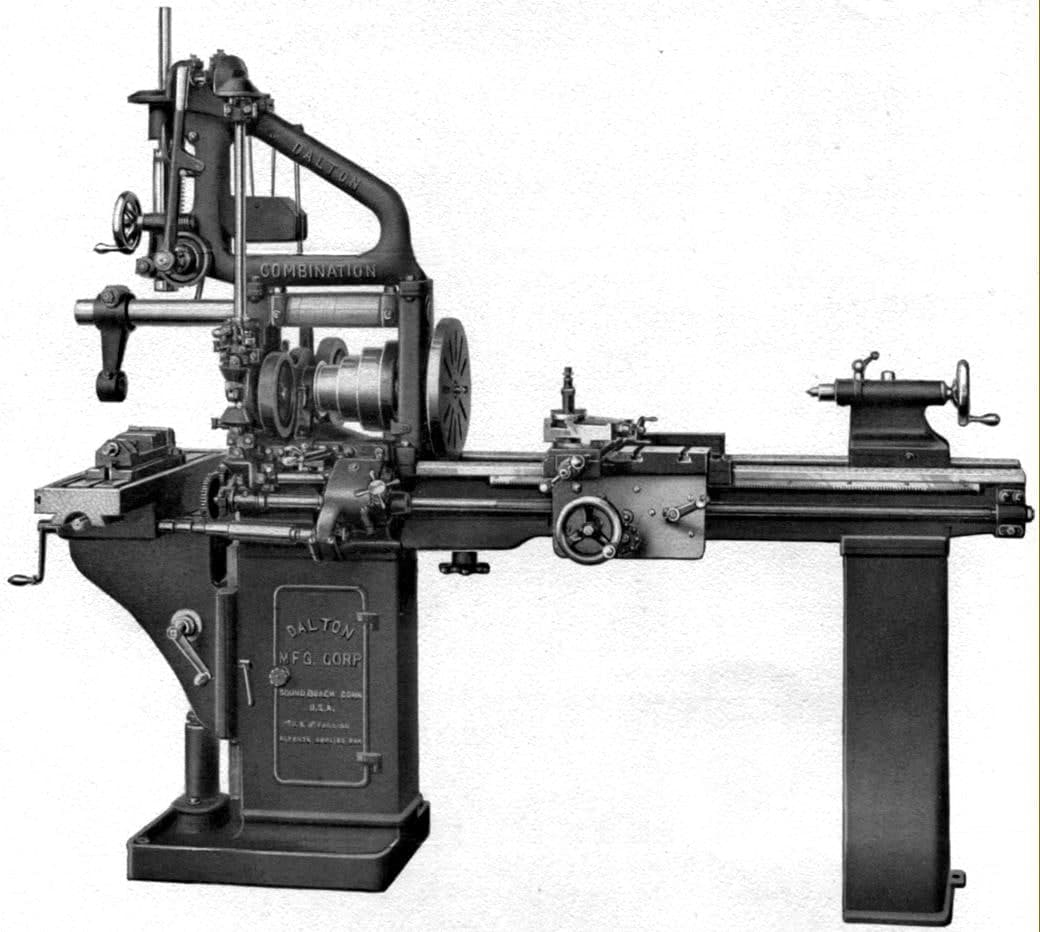
\includegraphics[width=0.7\textwidth]{ch-1/dalton}
	}
	\caption{Dalton Combinantion Machine.}\label{fig:dalton}
\end{figure}

\paragraph{Piho Combination Machine}

Piho Combination Machine "--- комбинированный универсальный станок, производимый в конце 1940-х годов компанией Hartensteiner Maschinenfabrik, рекламировался производителем как устройство, которое будет использоваться в ремонтных мастерских. Существовало два типоразмера: б\'ольшая версия имела возможность регулирования высоты заднего центра в диапазоне от 175 до 300\:мм и межцентровое расстояние равное 1300 мм; меньшая (настольная версия) "--- от 60 до 100\:мм и 180\:мм между центрами соответственно. Обе модификации могли работать как токарный станок, а также как горизонтальный и вертикальный фрезерный станок.

Несмотря на компромиссы, заложенные в конструкции, в станке были реализованы составные направляющие скольжения, низкоскоростной узел заднего редуктора, ходовой винт, движущийся под станиной, а также был оснащен барабаном для реверса шпинделя и тонкой подачей с ременным приводом. Очевидно, что в качестве токарного станка он работал так же, как и любой другой обычный токарный станок даже меньшего типоразмера. Однако наличие дополнительного фрезерного модуля, позволяло ему приблизится по своим возможностям к современным обрабатывающим центрам. Более того, фрезерный модуль был оснащен пинолью для быстрой подачей для сверления и имел возможность наклона в плоскости, перпендикулярной оси токарного станка. За счет большого размера расточного стола можно было ещё повысить универсальность станка, используя его в качестве горизонтального фрезерного.

\begin{figure}[ht]
	\centerfloat{
		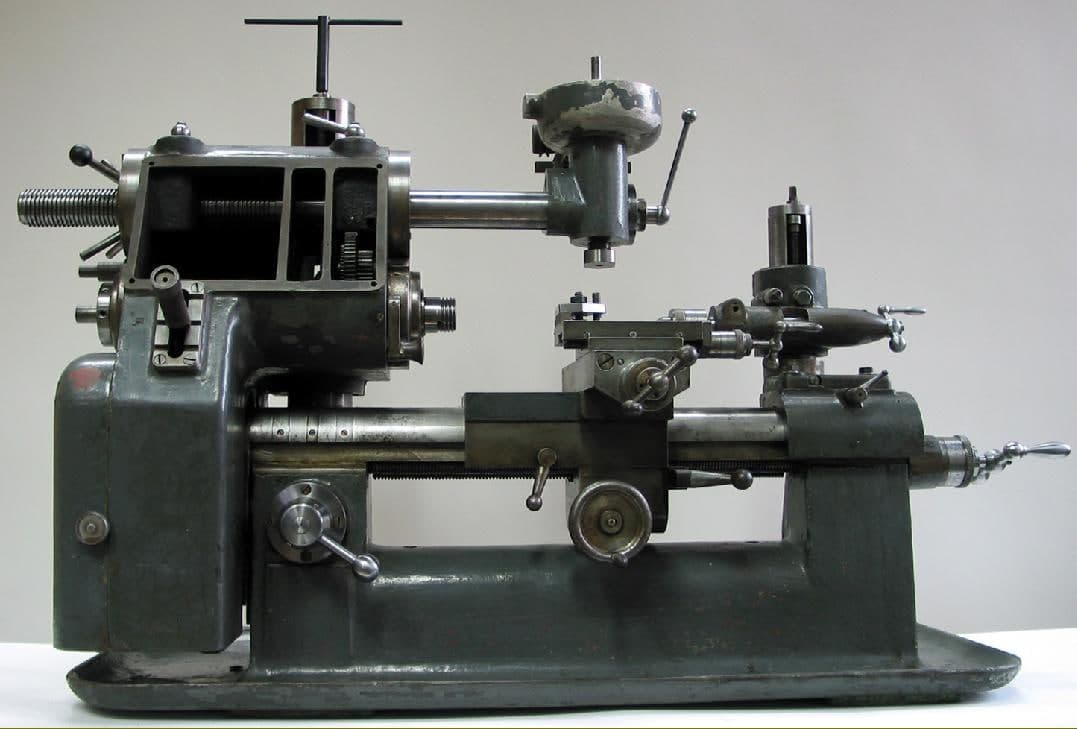
\includegraphics[width=0.7\textwidth]{ch-1/piho}
	}
	\caption{Piho Combination Machine.}\label{fig:piho}
\end{figure}

\paragraph{Adcock \& Shipley Combination Machine Tool}

<<Универсал>> Adcock \& Shipley обладал максимальной гибкостью и модульностью по сравнению с другими подобными станками. На площади всего 7 футов на 3 фута для б\'ольшей модели и 11 футов 6 дюймов на 3 фута 8 дюймов для меньшей помещались токарно-винторезный станок, круглошлифовальный станок для внутреннего и внешнего шлифования, вертикальный/горизонтальный фрезерный станок, а также сверлильный станок и специализированные модуля для заточки инструмента. Вместо выдвижных или подъемных станин и передней бабки, которые использовались на многих других станках того же типа, Ryder был построен на основе обычного токарного станка, причем каждый отдельный модуль имел автономный привод и мог (кроме шлифовального станка) работать параллельно с другими модулями. Устройство было первоначально разработано для использования на борту корабля и соответствовало различным требованиям, установленным Британским адмиралтейством для этой цели. 

\begin{figure}[ht]
	\centerfloat{
		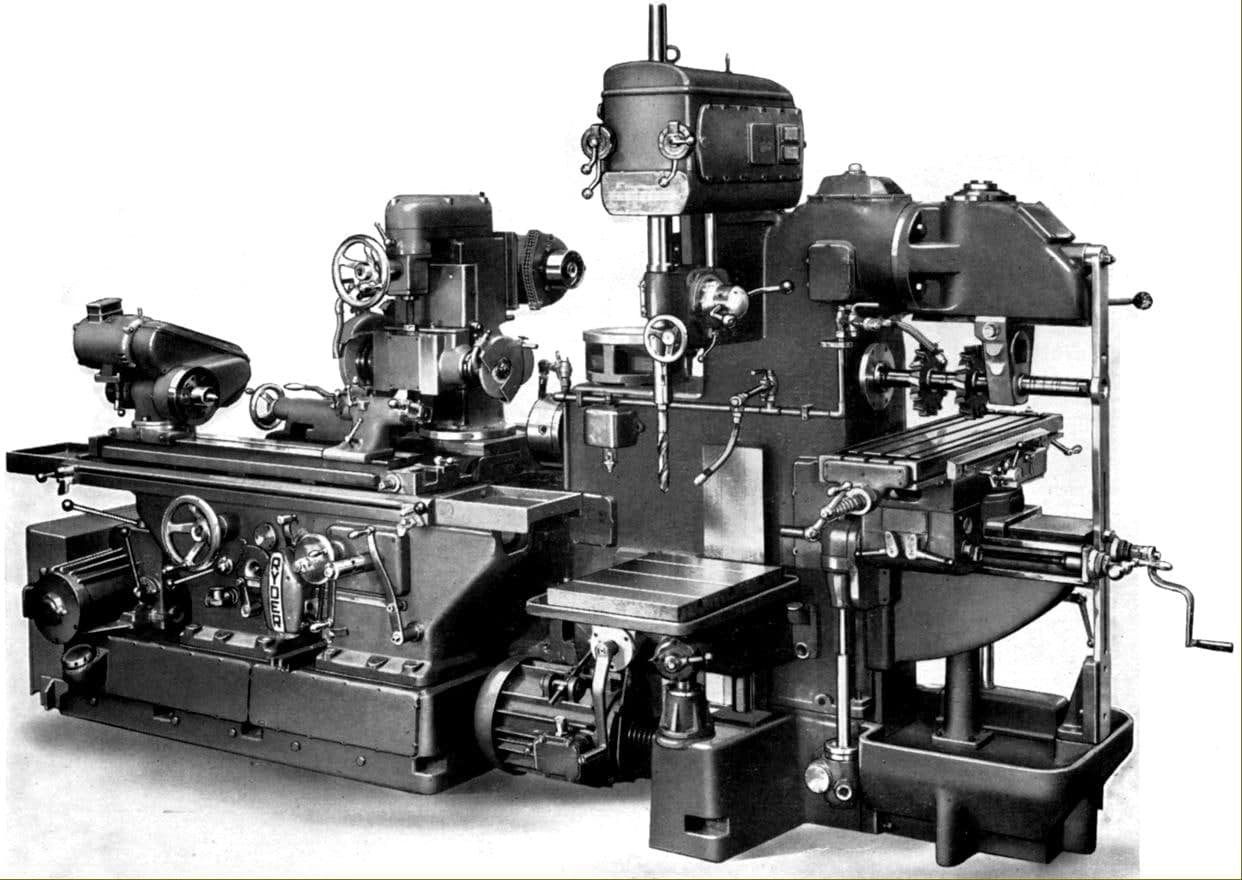
\includegraphics[width=0.7\textwidth]{ch-1/adcock-1}
	}
	\caption{Piho Combination Machine.}\label{fig:adcock-1}
\end{figure}

Токарный модуль обладал следующими характеристиками: высота над станиной 8 дюймов, расстояние между центрами 18 дюймов, коробка передач из 8 скоростей, обеспечивающая максимальную частоту вращения шпинделя в 1020 об/мин., трехфазный привод на 3 л.с., 1760 об/мин. Проходное отверстие шпинделя было всего 0,75 дюйма, что вряд ли соответствовало той работе, для выполнения которой мог бы потребоваться рассматриваемый станок. Также на станке был установлен упрощенный редуктор для нарезания резьбы с ходовым винтом, позволявшим нарезать дюймовые резьбы с шагом от 4 до 100 ниток на дюйм. Для автоподачи суппорта использовался отдельный ходовой вал, а ходовой винт был нужен исключительно для нарезания резьб.

Фрезерный модуль обладал оригинальной конструкцией с горизонтальным и вертикальным шпинделями. Рабочая поверхность фрезерного стола была размером 26 на 6 дюймов с продольным ходом 10 дюймов и поперечным всего 5,5 дюйма, вертикальный ход стола составлял 10 дюймов, что было крайне мало по сравнению со схожими по размерам универсальными фрезерными станками того времени. Оба шпиндели были рассчитаны на инструмент под конус ISO 40, горизонтальный мог вращаться с частотой от 48 до 970 об/мин, вертикальный "--- от 77 до 1575 об/мин.

Универсальный стол шлифовального станка с возможностью поворота на 45 градусов по часовой стрелке и 15 градусов против часовой стрелки был установлен параллельно станине токарного станка и использовался как опора для шлифовальной головки. Два зубчатых колеса соединяли головку с органами управления в передней части станка. Максимальная высота заготовки над столом составлял 7 дюймов, максимальная длина "--- 10 дюймов. Также была возможна заточка различного режущего инструмента. Подача охлаждающей жидкости к шлифовальной головке представляла собой отдельный блок, разработанный, чтобы избежать загрязнения другой охлаждающей жидкости (подаваемой на токарный, фрезерный и сверлильный модули) абразивными частицами.

Сверлиьлный модуль устанавливался на задней части <<шпиндельной бабки>> токарного станка и имел шесть скоростей от 420 до 5000 об/мин с мощностью, обеспечиваемой отдельным двигателем мощностью 0,5 л.с. Диапазон выбора инструмента был обусловлен использованием в патроне конуса Морзе 1, что ограничивало применение данного модуля для легких работ.

\begin{figure}[ht]
	\centerfloat{
		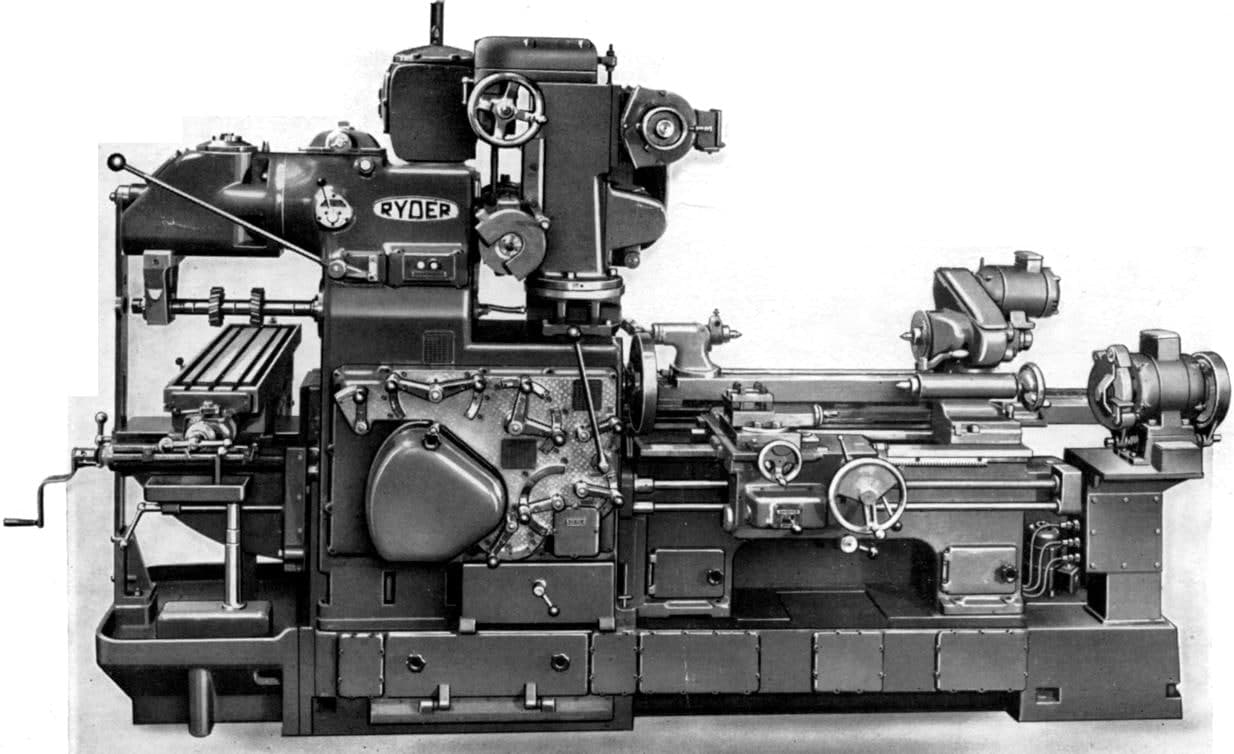
\includegraphics[width=0.7\textwidth]{ch-1/adcock-2}
	}
	\caption{Piho Combination Machine.}\label{fig:adcock-2adcock}
\end{figure}

\subsection{Агрегатные станки}

Агрегатными называются станки, которые компонуются из нормализованных и частично специальных узлов и деталей путем объединения их в единый агрегат (станок, рабочий комплекс) с общей системой управления и контроля. Агрегатные станки (АС) применяют в крупносерийном и массовом производстве. Все более широко применяются агрегатные станки с ЧПУ, используемые в серийном производстве. На агрегатных станках осуществляют многоинструментную и многопозиционную обработку деталей В начале развития агрегатных станков на них выполнялся только один какой-либо вид обработки (главным образом сверление и резьбонарезание) В настоящее время на агрегатных станках выполняются практически все технологические операции.

Агрегатные станки могут быть специальными и специализированными. Если первые могут обрабатывать одну или несколько деталей, но одновременно, то специализированные спроектированы для последовательной обработки нескольких деталей, требующей незначительной переналадки станка АС обычно выпускаются полуавтоматическими, а в составе автоматических линий "--- автоматическими.

Современные агрегатные станки с полуавтоматическим циклом работы начали применять в первой четверти ХХ\:в. в Германии для производства швейных машин, а позднее в США в автомобильной промышленности. В начале 1930-х гг. под руководством будущего академика В.\:И.\:Дикушина было начато проектирование и изготовление в СССР агрегатных станков. В 1934 г. был выпущен первый советский агрегатно-сверлильный станок для сверления отверстий в картере заднего моста грузового автомобиля.

Принцип агрегатирования основан на том, что вместо разработки всех узлов при проектировании нового станка используют ранее разработанные узлы, компонуя из них новый станок Для этого предварительно разрабатываются несколько однотипных узлов (агрегатов) разных размера и мощности (называются нормализованными или унифицированными), позволяющих спроектировать станок, довольно хорошо соответствующий технологическому процессу обработки детали. Кроме того, стараются эти агрегаты делать самодействующими, снабжая каждый своим двигателем. Агрегатные специальные станки имеют существенные преимущества перед другими станками:

\begin{itemize}
	\item возможность создания оборудования по наивыгоднейшему технологическому процессу Когда намечается применение агрегатных станков, сначала разрабатывают \item процесс обработки детали, а потом для выполнения этого процесса компонуют станки из готовых узлов;
	\item многоинструментная обработка, которая резко повышает производительность работы;
	\item возможность выполнения самых разных операций на одном станке;
	\item позволяют постоянно совершенствовать само оборудование, так как надо модернизировать не весь станок, а лишь тот узел, который устарел;
	\item создаются благоприятные условия для узлового ремонта станков;
	\item повышается надежность работы оборудования, созданного из проверенных нормализованных узлов;
	\item специальные станки собираются из серийных узлов, что их удешевляет.
\end{itemize}

Наряду с плюсами, у агрегатных станков есть и минусы, которые в последние годы сильно сократили спрос на эти станки даже для массового производства:

\begin{itemize}
	\item для новой детали, даже незначительно отличающейся от прежней по обрабатываемым поверхностям, надо делать новый специальный станок;
	\item станки стоят довольно дорого и имеют узкую область применения — массовое производство.
\end{itemize}

Для устранения этих противоречий надо, чтобы специальное станочное оборудование соответствовало трем главным условиям:

\begin{itemize}
	\item позволяло делать переналадку для обработки разных деталей при достаточно высокой производительности (это самое главное, потому что стоимость
	\item основных средств составляет значительную долю в себестоимости продукции);
	\item имело короткие сроки проектирования и изготовления;
	\item имело невысокую стоимость и быструю окупаемость.
\end{itemize}

В целом агрегатные станки в определенных условиях производства этим условиям отвечают. Унифицированными или нормализованными узлами агрегатных станков называются узлы, конструкции которых разрабатываются до того, как будет проектироваться конкретный станок. Эти узлы могут применяться в станках разных конструкций. К ним относятся станина, поворотный делительный стол, на котором устанавливаются приспособления и обрабатываемые детали, силовые бабки. Для установки на станке силовых головок служат боковые станины, стойки, проставочные плиты. При многошпиндельной обработке отверстий или при фрезеровании плоскостей к силовым головкам крепят сверлильные и фрезерные насадки. Управление станком сосредоточено на пульте, а вся электроаппаратура размещается в шкафу. Из нормализованных сборочных единиц конструируют специальные узлы, компонуя их так, как того требует конструкция обрабатываемой детали. Типаж унифицированных узлов включает несколько сотен наименований более 2500 исполнений и типоразмеров и составляет 75--80\% узлов станка.

В агрегатных станках количество силовых узлов и инструментальных шпинделей, расположение осей шпинделей зависят от реализуемого на станке технологического процесса. Различают станки одноагрегатные и многоагрегатные, одношпиндельные и многошпиндельные, горизонтальные, вертикальные, наклонные и комбинированные, односторонние и многосторонние.

На однопозиционных станках обработка полностью заканчивается при постоянном положении детали На многопозиционных станках с поворотно-делительными столами обработка деталей выполняется параллельно или последовательно на нескольких позициях в разных положениях относительно инструментов.

Агрегатные станки можно оснастить загрузочными приспособлениями, и они станут автоматами. АС работают как самостоятельно, так и в составе автоматических линий.

Силовые головки агрегатных станков — это основные нормализованные узлы, определяющие их технологические возможности. Силовые головки предназначены для сообщения инструменту главного движения, рабочей подачи и установочных перемещений при сверлении, зенкеровании, развертывании и растачивании деталей из различных материалов. В большинстве случаев осуществляются циклы движений, включающие быстрый подвод инструмента, рабочую подачу (одну или две в зависимости от технологического процесса), выдержку на жестком упоре (при необходимости), быстрый отвод и остановку в конце хода. Программа движений может быть разной и осуществляется автоматически от кулачка, установленного внутри корпуса головки.

Основными параметрами силовых головок, которые характеризуют их технологические возможности и служат основанием для выбора конструкции силовых узлов, являются мощность привода главного движения, наибольшая сила подачи, частота вращения приводного вала шпинделя головки, пределы подач, скорость быстрых перемещений, длина рабочего хода, точность переключения механизма подачи, габаритные размеры.

Для выполнения операций, требующих больших затрат мощности: фрезерования, растачивания, подрезки больших торцов, — от силовых головок требуется повышенная жесткость. Описанные ранее силовые головки не отвечают этому требованию. Для повышения жесткости пришлось изменить конструкцию: механизм главного движения отделили от механизма подачи, и получились два узла — силовой стол и силовая бабка. 

Кроме устройств для прямолинейного перемещения, в агрегатных станках очень часто применяются поворотные делительные столы, предназначенные для закрепления на них приспособлений с заготовками и периодического поворота на определенный угол. Эти столы перемещают обрабатываемые детали из одной рабочей позиции в другую и, что очень важно, точно фиксируют заготовку относительно режущих инструментов. Столы поворачиваются в горизонтальной и вертикальной плоскостях. Делительные столы чаще всего выполняют дискообразными или кольцевыми с поворотом в горизонтальной плоскости, а также под названием «барабан» — для поворота в вертикальной плоскости. В последнем случае приспособления с деталями располагаются на периферии барабана и деталь можно одновременно обрабатывать с двух сторон.

Электромеханический поворотный делительный стол состоит из собственно стола (планшайбы), основания и редуктора. Нижней плоскостью стол установлен на привалочную плоскость станины. В качестве механизма поворота используются разные устройства. Это может быть мальтийский механизм или какой-то другой привод. Но обязательным условием является наличие узлов поворота, ориентации в нужном положении и устройства фиксации.

\section{Модульные системы управления технологическим оборудованием}\label{sec:ch1/sec2}

Анализируя развитие современной промышленности, можно прийти к выводу о том, что на сегодняшний день наиболее перспективным направлением развития в этой области является создание гибких распределенных автоматизированных производственных линий. Четвертая промышленная революция и постепенное внедрение кибер-физических производственных систем по-новому определяют само понятие массового производства.

Происходит последовательный переход от <<жестких>> конвейерных решений к малым партиям, выполняемым по индивидуальным заказам. Также не останавливается развитие  концепции малых инновационных предприятий и стартапов. Все это приводит к изменению подхода к проектированию современного интеллектуального оборудования. 

Первые станки с ЧПУ появились еще в 50-х годах прошлого века, и с тех пор их развитие не прекращается. Тем не менее, вектор этого развития всегда был ориентирован исключительно на массовое производство. Системы с ЧПУ всегда были и остаются сложными, высокопроизводительными, а самое главное "--- очень дорогим. Процесс внедрения подобных систем очень долог, а время жизни современных автоматизированных производств может исчисляться десятилетиями.

Конечно, все это усложняет внедрение современных коммуникационных технологий. Любое изменение требует либо полного перестроения устоявшейся производственной системы, либо создания дополнительного слоя управления, который позволит связать устаревшее оборудование с современной кибер-физической системой.

Такой подход представляется наиболее целесообразным в переходный период, но в дальнейшем от него, безусловно, придется отказаться. Необходим пересмотр самой парадигмы проектирования оборудования с ЧПУ. Нужно рассматривать любое новое оборудование с точки зрения возможности включения его в единую информационно-телекоммуникационную среду с использование открытого протокола.

Попытки реализации подобного подхода делались уже неоднократно. Например, в работе Grigoriev and Martinov предлагается подход к построению переносимого ядра ЧПУ на основе платформы независимых библиотек. Открытая архитектура данной системы ЧПУ включает в себя уровни абстракции для реализации различных человеко-машинных интерфейсов, а также имеет возможность описания компонентов системы на различных языках программирования. Компоненты системы связываются между собой по шине Fieldbus
%~\cite{grigoriev2014research}
.
Bin et al. описывают открытую платформу для создания систем ЧПУ. Данная система состоит из набора универсальных компонентов, которые могут быть использованы повторно, а также коммуникационных модулей для их связи%
%\cite{bin2004research}

.

Morales-Velazquez et al. предлагают платформу с открытой архитектурой на основе многоагентной системы программно-аппаратных компонентов, именуемой MADCON. The Аппаратные блоки предлагаемой системы объединяют функции управления и мониторинга, обеспечивая открытую архитектуру на базе FPGA для реконфигурируемых приложений. Компоненты программного обеспечения используют структуру XML для файлов описания системы, собирая такие функции, как язык описания блок-схем и графический интерфейс пользовател/я%~\cite{morales2010open} 

В работах Verba et. al
%~\cite{verba2017platform}
и  Prazeres and Serrano
%~\cite{prazeres2016soft}
рассматривается очень интересная концепция Fog of Things. Данная концепция является развитие концепции Internet of Things, являющейся основой многих кибер-физических производственных систем. Fog of Things позволяет создать более однородную информационно-телекоммуникационную среду за счет совершенствования и упрощения протокола взаимодействия компонентов.

В работе [morales2010open] представлена система ЧПУ с открытой архитектурой, основанная на авторской мультиагентной аппаратно-программной платформе Multi-Agent Distributed CONtroller (MADCON). Эта система имеет возможность реконфигурируемости и адаптивности. При проектировании интеллектуальных приводов для этой системы были использован структурированный подход к созданию программных и аппаратных составляющих. Аппаратные блоки предлагаемой системы объединяют в себе функции управления и мониторинга, обеспечивая открытую архитектуру на основе ПЛИС для обеспечения реконфигурируемости. С другой стороны, программные компоненты разработаны с использованием языка XML для описания системы, что позволило отказаться от привычного программирования и создавать логику программных компонентов с помощью визуальных блок-схем. MADCON был применен в качестве системы управления модернизированным токарным станком с ЧПУ для управления и контроля с целью проверки предлагаемой архитектура, которая может быть применена для создания интеллектуального производства нового поколения системы.

В [han2007development] рассматривается контроллер с открытой архитектурой, который может стать основой для различного оборудования с ЧПУ. Разрабатываемый контроллер имеет модульную арихтектуру, а в качестве аппаратной платформы использует персональный компьютер. Основная цель работы "--- разработать методику построения программно-аппаратная платформа системы ЧПУ. Также исследуются методы статического моделирования контроллера с открытой архитектурой, включающие технологию объектно-ориентированного программирования, технологию применения динамических библиотеки и разделения системных модулей. Авторы обсуждают динамическое моделирование поведения и представление потока данных контроллера с открытой архитектурой, которые описаны с помощью иерархической модели конечного автомата. Для разработки библиотеки программных функциональных компонентов авторы создали модель многократно используемого программного модуля. В качестве испытательного стенд выступает 3-осевой фрезерный станок. Для данного станка был успешно разработан программный код системы ЧПУ, основанной на описанной библиотеке функциональных модулей с применением методики конфигурирования системы. Результаты экспериментов показывали, что, помимо увеличения степени повторного использования программного кода и открытости, применение вышеупомянутой методологии приводит к значительному сокращению времени разработки, а также стоимости обслуживания конечного оборудования с ЧПУ.

\section{Современные тенденции в области стандартизации модульного оборудования}


\section{Название раздела}\label{sec:ch1/sec3}

\subsection{Название подраздела}\label{subsec:ch1/sec3/sub1}

\subsection{Название подраздела}\label{subsec:ch1/sec3/sub2}

\subsection{Название подраздела}\label{subsec:ch1/sec3/sub3}

\subsection{Название подраздела}\label{subsec:ch1/sec3/sub4}

\section{Выводы по главе 1}

\FloatBarrier
